\section{Excavation System Mass}
The general function of an excavation system is to interact with an asteroid, contain an amount of asteroid material, and deliver that material to a processing system. There are numerous ways to accomplish this task, such as having separate small excavation spacecrafts gather asteroid material and deliver it to a mother processing spacecraft. However, from a first principals modelling viewpoint the specifics of the excavation method are not particularly relevant. 
\newline
This model assumes a single, large container is used to interact with the asteroid and contain the asteroid material. This is the principal component of the excavation system. Motors, material transfer mechanisms, and other auxiliary equipments are modelled by a constant mass offset and a linear margin.
\newline 
The first calculation is to determine the amount of asteroid material the excavation system needs to gather. This model is based on processing water, so a target water mass in kg is the initial input. Some variable names have been changed from what they are in the python model for readability and clarity in this document. 
\begin{equation}
    m_{asteroid} = m_{waterTarget} / x_{asteroid water percent}
\end{equation}

This mass needs to be converted into a volume:
\begin{equation}
    V_{asteroid} = m_{asteroid} / density_{asteroid}
\end{equation}

It may be more practical to have an excavation system that takes several excavation passes at the asteroid. This would allow for a lower overhead excavation system volume and mass.
\begin{equation}
    V_{excavation} = V_{asteroid} / n_{number of excavation scoops}
\end{equation}

The shape of the excavation container (cube, cylinder, sphere) determines the relationship between the contained volume and the surface area needed to contain that volume. This relationship is modelled below:
\begin{equation}
    SA/V = SAtoV_{factor} / V_{excavation}^{1/3}
\end{equation}
\begin{equation}
    SA_{excavation} = SA/V \cdot V_{excavation}
\end{equation}

The surface area needed to contain the asteroid material is used to calculate the mass of the excavation container.
\begin{equation}
    m_{excavationContainer} = SA_{excavation} \cdot material_{thickness} \cdot material_{density}
\end{equation}

The total mass of the excavation system is then 
\begin{equation}
    m_{excavation} = m_{excavation offset} + m_{container} \cdot containerMass_{factor}
\end{equation}

The output to these equations over a range of water targets is shown in \autoref{fig-exmass}. The inputs are varied within the larger model, this figure is meant to show the deterministic model behavior with respect to excavation mass.
\begin{figure}[htb]
    \centering
    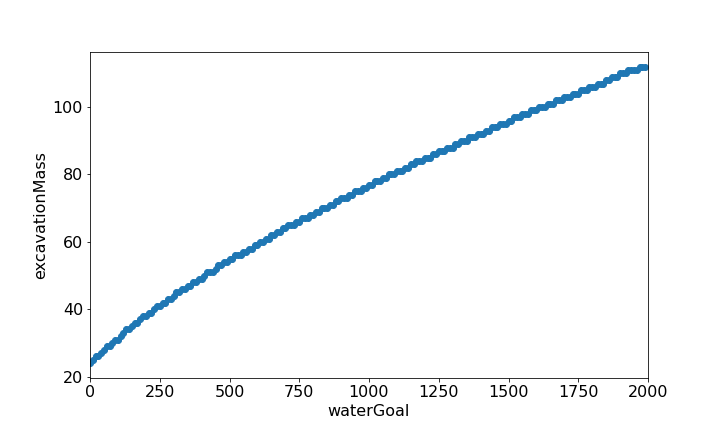
\includegraphics[width=0.5\linewidth]{exMass_vs_waterGoal.png}
    \caption{Excavation mass calculation for range of target water masses. Both values are in kilograms.}
    \label{fig-exmass}
\end{figure}
